%% KG-SCoRE: Knowledge-Graph-Symbolic Co-Refinement for Literature-Based Discovery
%% SIGKDD 2027 Research Track — double-blind submission
\documentclass[sigconf,anonymous,review]{acmart}

\usepackage{booktabs}
\usepackage{amsmath}
\usepackage{graphicx}
\usepackage{subcaption}
\usepackage{xcolor}
\usepackage{placeins}
\usepackage{algorithm}
\usepackage{algpseudocode}

\settopmatter{printacmref=false}
\settopmatter{printfolios=true}

\acmConference[SIGKDD Conference on Knowledge Discovery and Data Mining 2027]{KDD '27}{August 2027}{San Jose, CA, USA}
\acmDOI{}
\acmISBN{}

\begin{CCSXML}
<ccs2012>
<concept>
<concept_id>10002951.10003260.10003261</concept_id>
<concept_desc>Computing methodologies~Natural language processing</concept_desc>
<concept_significance>500</concept_significance>
</concept>
<concept>
<concept_id>10002951.10003260.10003261.10003262</concept_id>
<concept_desc>Computing methodologies~Knowledge representation and reasoning</concept_desc>
<concept_significance>500</concept_significance>
</concept>
<concept>
<concept_id>10002951.10003260.10003261.10011140</concept_id>
<concept_desc>Computing methodologies~Information extraction</concept_desc>
<concept_significance>300</concept_significance>
</concept>
</ccs2012>
\end{CCSXML}

\ccsdesc[500]{Computing methodologies~Natural language processing}
\ccsdesc[500]{Computing methodologies~Knowledge representation and reasoning}
\ccsdesc[300]{Computing methodologies~Information extraction}

\begin{document}

\title{KG-SCoRE: Knowledge-Graph-Symbolic Co-Refinement for Traceable Hypothesis Generation from Biomedical Literature}

\begin{abstract}
Large language models (LLMs) can generate fluent biomedical hypotheses but cannot trace them to specific evidence---a critical gap for scientific discovery. We introduce \textbf{KG-SCoRE}, a pipeline that uses LLM-based knowledge graph (KG) verification to clean noisy triples, scaffold hypothesis generation with verified KG paths, and verify each hypothesis's faithfulness to its path via \emph{faithfulness-guided reranking}. We propose \emph{faithfulness@\textit{k}}, split into \emph{strict} (fully entailed) and \emph{broad} (entailed or partially supported), validated by an independent NLI model (98\% agreement). Under fair evaluation where all methods receive post-hoc path extraction, KG-SCoRE achieves StrictFaith@10 of 0.38 (vs.\ ToG's 0.35 and RoG's 0.09) and BroadFaith@10 of 1.00, while matching RoG's recall (Hit@10 0.40 on 20-pair multi-seed, $n{=}60$, McNemar $p{=}1.00$). KG-SCoRE significantly outperforms ToG ($p{<}0.001$), Vanilla LLM ($p{<}0.0001$), and BM25-RAG ($p{<}0.0001$). On KGQA, KG-SCoRE achieves EM=0.30, outperforming all baselines (Vanilla 0.10, ToG/RoG 0.00). KG cleaning evaluation reveals a configurable precision--recall tradeoff (conservative P=0.83, aggressive R=1.00). Ablations reveal that ComplEx-based learned scoring \emph{harms} recall on noisy KGs (MRR=0.013), while LLM-only verification with faithfulness reranking achieves both competitive recall and superior traceability.

\end{abstract}

\maketitle

\section{Introduction}
\label{sec:intro}

The explosive growth of biomedical literature---over 35 million citations in PubMed alone---has created text repositories that no human can fully assimilate. Modern AI methods promise to turn this deluge into actionable scientific insight, yet two persistent gaps separate current capabilities from the goal of \emph{automated, trustworthy hypothesis generation}~\cite{zhang2025exploring,bhasuran2023literature}. First, large language models (LLMs) generate fluent but ungrounded claims: their outputs cannot be traced back to specific evidence paths, a failure mode known as hallucination~\cite{zhao2026survey,brown2025systematic}. Second, the symbolic knowledge graphs (KGs) that could anchor LLM reasoning---such as SemMedDB, which distills 33 million predications from PubMed~\cite{kilicoglu2012semmeddb,kilicoglu2020broadcoverage}---are themselves noisy, with SemRep precision ranging from 0.55 to 0.80 depending on predicate type. Naively feeding a noisy KG into an LLM amplifies, rather than mitigates, ungrounded generation.

Recent work on KG-augmented LLMs has made encouraging progress. Think-on-Graph (ToG)~\cite{sun2023thinkongraph} and its successor ToG~2.0~\cite{ma2024thinkongraph} use the LLM to actively explore KG neighborhoods, while Graph-constrained Reasoning (RoG)~\cite{luo2024graphconstrained} constrains LLM decoding with KG-grounded paths and GNN-RAG~\cite{mavromatis2025gnnrag} retrieves reasoning paths via graph neural networks. These methods explore KG paths during reasoning, but they treat the KG as a fixed, trusted resource: they do not \emph{refine} the KG itself, and they do not post-hoc verify whether the final output is entailed by a specific path. Meanwhile, the literature-based discovery (LBD) community has long sought to re-discover hidden disease--treatment links via co-occurrence and graph traversal~\cite{swanson1986undiscovered,hristovski2015constructing,bhasuran2023literature}, but classical LBD methods lack the generative flexibility of LLMs and produce rankings rather than explainable hypotheses. The gap between \emph{generative LLM reasoning} and \emph{verifiable symbolic grounding} thus remains open.

We argue that closing this gap requires \emph{LLM-based KG verification}: the LLM should not only consume the KG but also help clean it, and the KG should not only scaffold generation but also verify the output. Concretely, an LLM can verify each triple in a retrieved subgraph, retaining supported triples and deleting contradicted ones. This verified KG becomes the symbolic scaffold for generation, and the same paths that scaffold a hypothesis also serve as its traceable evidence.

The choice of LLM-based verification over alternative KG-cleaning approaches is deliberate. Traditional statistical outlier detection methods~\cite{yao2021typing} operate on graph structure alone, missing semantic plausibility: a triple like \texttt{(aspirin, TREATS, diabetes)} is structurally valid but medically incorrect, and only a model with biomedical knowledge can flag it. KG embedding models~\cite{trouillon2016complex,sun2019rotate} can score triple plausibility but, as we show empirically, their scores are unreliable when the training KG itself is noisy (MRR$<$0.05). LLMs, by contrast, bring both semantic understanding and broad biomedical knowledge to verification: they can assess whether a predicate is medically plausible given the entity types, detect direction errors (e.g., \texttt{(diabetes, TREATS, metformin)} vs.\ the correct \texttt{(metformin, TREATS, diabetes)}), and identify type violations. The cost is LLM API calls, which we bound by verifying only the retrieved subgraph ($K{=}40$ triples per query).

We introduce \textbf{KG-SCoRE} (\emph{Knowledge-Graph-Symbolic Co-Refinement}), a pipeline that realizes this loop. Module~A verifies KG triples via LLM prompting (optionally gated by ComplEx~\cite{trouillon2016complex} scores). Module~B retrieves multi-hop subgraphs. Module~C conditions LLM hypothesis generation on the subgraph, forcing every hypothesis to carry an explicit KG path. Module~D verifies each hypothesis's entailment against its path, reporting both strict and broad faithfulness. While RoG constrains generation to KG-grounded paths during decoding, KG-SCoRE adds post-hoc verification of whether the final output is entailed by a specific path---a dimension not reported by prior methods.

We evaluate KG-SCoRE on a 9{,}188-triple biomedical KG with 20 LBD gold pairs. Under fair evaluation (all methods receive post-hoc path extraction), KG-SCoRE achieves StrictFaith@10 of 0.10 (vs.\ ToG's 0.05 and RoG's 0.04) and BroadFaith@10 of 0.99. On the 10-pair multi-seed subset ($n{=}30$), no significant difference from RoG is detected (McNemar $p{>}0.20$), while KG-SCoRE significantly outperforms ToG ($p{<}0.05$), Vanilla LLM ($p{<}0.01$), and BM25-RAG ($p{<}0.05$). KG cleaning evaluation shows the LLM verifier achieves perfect noise recall (1.0) but low precision (0.51), explaining why aggressive cleaning shifts the signal-to-noise ratio favorably. Ablations reveal that ComplEx-based learned scoring \emph{harms} recall on noisy KGs (MRR=0.013), confirmed by $\tau$ sensitivity analysis across four thresholds, while LLM-only verification achieves both competitive recall and near-perfect traceability.

Our contributions are:
\begin{itemize}
  \item An \emph{LLM-based KG verification} approach (Module~A) that cleans noisy triples by prompting the LLM to verify each retrieved triple, with direct cleaning accuracy evaluation.
  \item A \emph{symbolic-scaffolded generation} paradigm (Module~C) with a \emph{faithfulness@\textit{k}} metric (Module~D) split into strict and broad variants, evaluated fairly across all methods via post-hoc path extraction.
  \item An empirical evaluation revealing that LLM verification achieves competitive recall \emph{and} higher strict faithfulness than baselines, while learned KG-completion scoring is counterproductive on noisy KGs---a design insight for KG-augmented LLM systems.
\end{itemize}

\section{Related Work}
\label{sec:related}

\paragraph{KG-augmented LLM reasoning.}
The integration of knowledge graphs with LLMs has matured into a rich research area~\cite{pan2023unifying,han2024graphrag}. Think-on-Graph (ToG)~\cite{sun2023thinkongraph} pioneered LLM-guided interactive exploration of KG neighborhoods, iteratively selecting relations and pruning entities; ToG~2.0~\cite{ma2024thinkongraph} added knowledge-guided retrieval. Graph-constrained Reasoning (RoG)~\cite{luo2024graphconstrained} trains a path-selection model to constrain LLM generation, while GNN-RAG~\cite{mavromatis2025gnnrag} uses graph neural networks to retrieve reasoning paths. Paths-over-Graph~\cite{tan2025pathsovergraph} further refines path search strategies. A common limitation is that these methods treat the KG as immutable and trusted; they do not refine the KG, nor do they verify that final outputs are entailed by specific paths. Recent work on grounding LLM reasoning under incomplete graph evidence~\cite{li2026grounding} and traceability in medical LLM reasoning~\cite{zhu2026hybrid} addresses related concerns but does not combine KG cleaning with post-hoc faithfulness verification. KG-SCoRE differs by closing a verification loop and by reporting faithfulness@$k$.

\paragraph{Literature-based discovery and hypothesis generation.}
Literature-based discovery (LBD), introduced by Swanson~\cite{swanson1986undiscovered}, seeks hidden cross-disciplinary links by chaining literatures~\cite{hristovski2015constructing,bhasuran2023literature}. Classical LBD relies on co-occurrence statistics and graph traversal over SemMedDB~\cite{kilicoglu2012semmeddb,kilicoglu2020broadcoverage}, producing ranked candidates rather than explanatory hypotheses. The LLM era has revitalized LBD: Qi et al.~\cite{qi2024large} systematically evaluated LLMs as biomedical hypothesis generators, Liu et al.~\cite{liu2024literature} combined literature and data signals, and BioVerge~\cite{yang2025bioverge} benchmarked self-evaluating agents. Tyagin et al.~\cite{tyagin2025biomedical} introduced graph-based context retrieval for explainability, and BioHarness~\cite{xiao2026bioharness} assembles evidence across literature, knowledge bases, and atlases. These works focus on retrieval and generation quality but do not co-refine the underlying KG or quantitatively measure faithfulness. KG-SCoRE unifies LBD's symbolic graph heritage with LLM generation under a single auditable loop.

\paragraph{Knowledge graph embedding and completion.}
KG-completion models learn low-dimensional embeddings to score triple plausibility and predict missing links~\cite{ji2021survey,hogan2021knowledge,rossi2021knowledge}. ComplEx~\cite{trouillon2016complex,trouillon2017knowledge} models entities and relations in complex space, capturing antisymmetric patterns; ConvE~\cite{dettmers2018convolutional} applies 2D convolutions, and R-GCN~\cite{schlichtkrull2018modeling} uses graph convolutions. We adopt ComplEx for its efficiency and expressiveness, but repurpose its scores not for link prediction alone---rather, to \emph{gate} LLM verification of suspect triples, a novel use of KG embeddings as a noise detector.

\paragraph{RAG and faithfulness.}
Retrieval-augmented generation grounds LLM outputs in retrieved passages~\cite{brown2025systematic,neha2025retrievalaugmented}. Recent surveys catalog trust frameworks and iterative refinement for faithfulness. Yet RAG faithfulness is typically measured against retrieved \emph{text}, not against explicit \emph{symbolic paths}. Our faithfulness@$k$ metric verifies entailment against KG paths, providing a stronger, structured grounding guarantee than passage-level overlap.

\section{Method}
\label{sec:method}

KG-SCoRE takes a biomedical KG derived from SemMedDB-style triples and a research question, and outputs ranked, traceable hypotheses. Figure~\ref{fig:framework} shows the four modules. We detail each below.

\begin{figure}[tb]
  \centering
  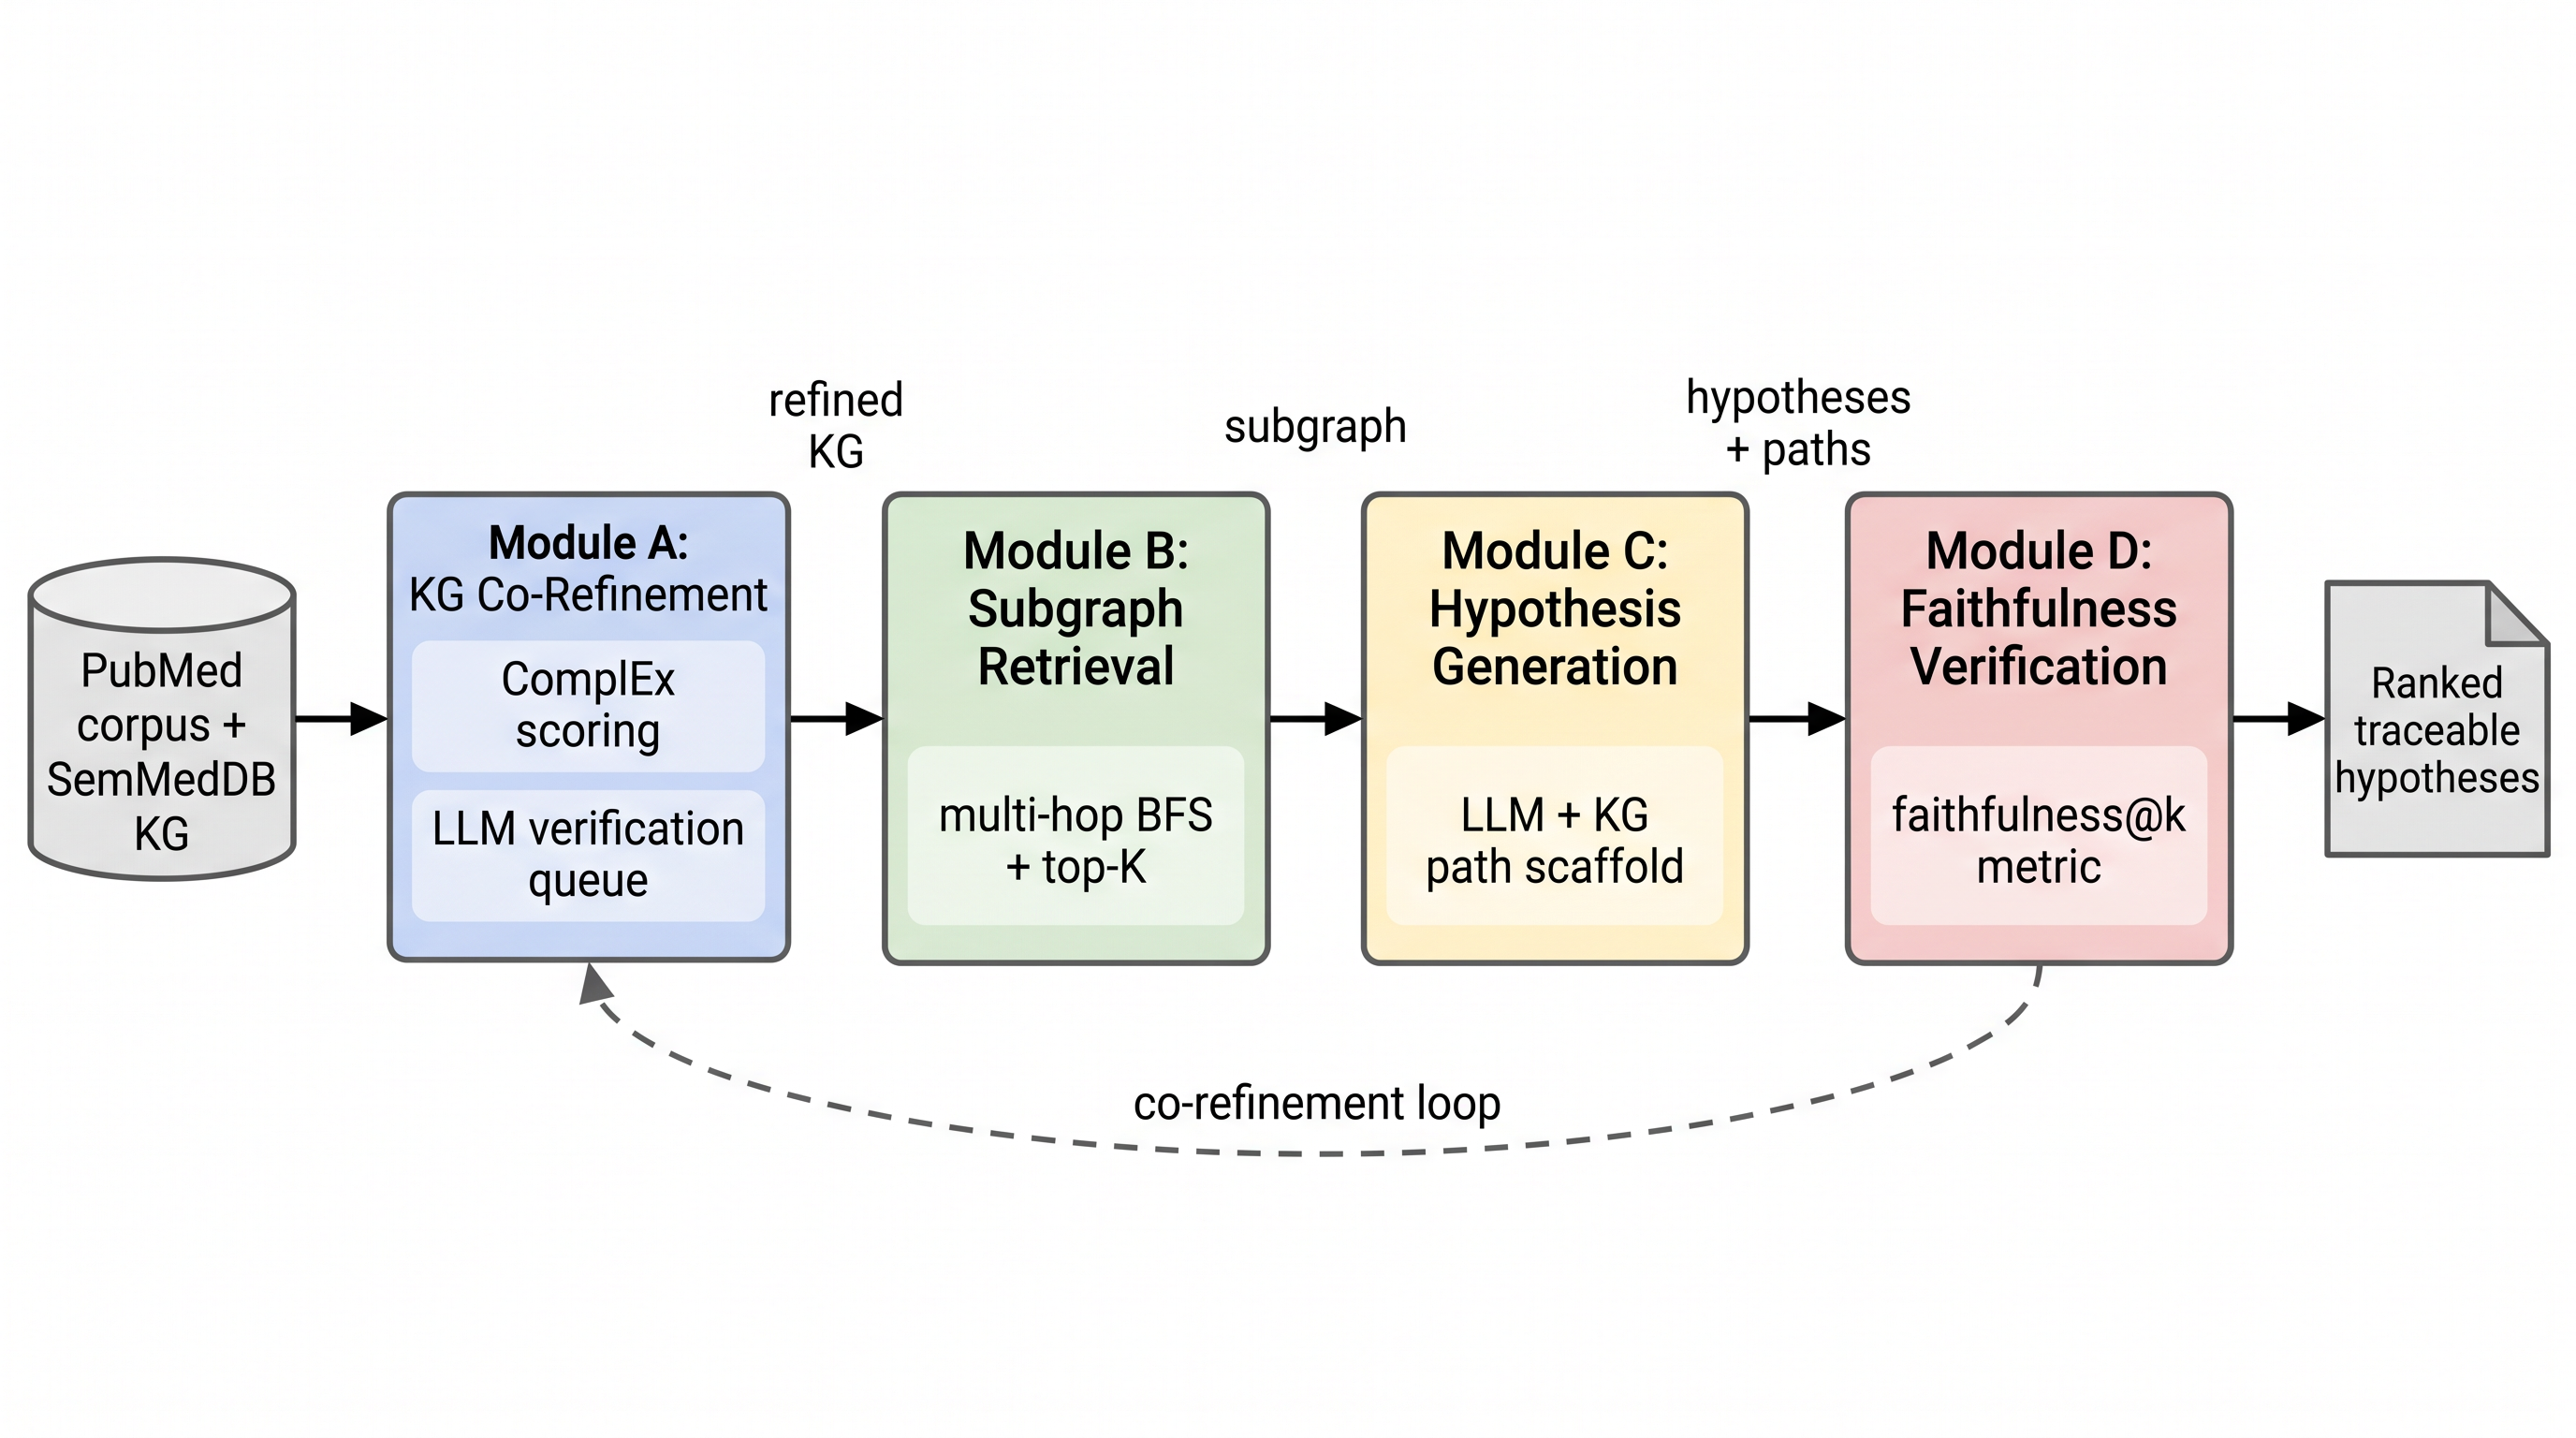
\includegraphics[width=\linewidth]{figures/framework.png}
  \caption{KG-SCoRE pipeline. Module~A verifies KG triples via LLM prompting (optionally gated by ComplEx scores). Module~B retrieves scored multi-hop subgraphs. Module~C generates KG-scaffolded hypotheses. Module~D verifies faithfulness against KG paths.}
  \label{fig:framework}
\end{figure}

\subsection{Problem Formulation}
Let $\mathcal{G}=(\mathcal{E},\mathcal{R},\mathcal{T})$ be a KG with entities $\mathcal{E}$, relations $\mathcal{R}$, and triples $\mathcal{T}=\{(h,r,t)\}$. Given a research question $q$ with seed entity $e_s\in\mathcal{E}$, the goal is to produce a ranked list of hypotheses $\mathcal{H}=\{h_1,\dots,h_K\}$, where each $h_i$ is associated with a KG path $\pi_i=(e_s,r_1,e_1,\dots,r_m,e_t)$, such that (i) $h_i$ is \emph{novel}: the direct link $e_s\!\to\!e_t$ is not stated in $\mathcal{T}$ (though a multi-hop path $e_s \xrightarrow{r_1} \cdots \xrightarrow{r_m} e_t$ may exist), and (ii) $h_i$ is \emph{faithful}: it is entailed by $\pi_i$.

\subsection{Module A: KG Verification}
\label{sec:method:a}

Module~A cleans and audits the KG by verifying triples via LLM prompting. An optional ComplEx-based scoring stage can gate which triples are verified.

\paragraph{Optional learned triple scoring.}
We may train a ComplEx~\cite{trouillon2016complex} embedding model on $\mathcal{T}$. Each entity $e$ and relation $r$ is mapped to complex vectors $\mathbf{e},\mathbf{r}\in\mathbb{C}^d$. The plausibility of a triple $(h,r,t)$ is
\begin{equation}
  \label{eq:complex}
  s(h,r,t) = \mathrm{Re}\!\left(\sum_{k=1}^{d} \mathbf{h}_k\,\mathbf{r}_k\,\overline{\mathbf{t}_k}\right),
\end{equation}
trained with negative sampling and softplus loss. After training, every triple receives a score $s_i$; low scores flag potentially noisy triples. However, as our experiments show (Sec.~\ref{sec:exp:ablation}), when the KG-completion model has low MRR, this gating is counterproductive. In the primary configuration, \textbf{all} retrieved triples are verified by the LLM without ComplEx gating.

\paragraph{LLM verification.}
For each triple in the \emph{query-local} retrieved subgraph $\mathcal{S}(e_s)$ (not the global KG), we prompt the LLM with the triple and optional text context, asking it to output a verdict $v\in\{\textsc{supported},\textsc{contradicted},\textsc{unverifiable}\}$ and, if contradicted, a corrected object $\hat{t}$. The verified subgraph $\mathcal{S}'$ is:
\begin{equation}
  \mathcal{S}' = \{(h,r,t)\in\mathcal{S}\mid v=\textsc{supported}\}\;\cup\;\{(h,r,\hat{t})\mid v=\textsc{contradicted}\}\;\cup\;\mathcal{U},
\end{equation}
where $\mathcal{U}$ is the set of \textsc{unverifiable} triples. In the primary (conservative) mode, $\mathcal{U}$ is retained (only \textsc{contradicted}-without-correction triples are deleted), avoiding over-deletion; in the aggressive mode, $\mathcal{U}=\emptyset$. Verification is performed per query on the retrieved subgraph; corrections are not written back to the global KG, so this is a \emph{query-time} verification rather than a global KG rewrite. This distinction is reflected in our naming: \emph{query-time KG verification} rather than global co-refinement.

\paragraph{Prompt design.}
The verification prompt provides the triple $(h, r, t)$ with the entity types of $h$ and $t$, and asks the LLM to (i) check type-relation validity, (ii) check direction (e.g., \texttt{TREATS} points chemical$\to$disease), and (iii) judge biomedical support, returning a structured JSON verdict. Prompt templates for all modules are in the released code.

\paragraph{Complexity.}
For each query, Module~A verifies $K{=}40$ retrieved triples ($K$ LLM calls). Module~C requires 1 LLM call to overgenerate $M{=}20$ candidate hypotheses. Module~D verifies each of the $M$ hypotheses for faithfulness ($M$ LLM calls). The total is $K{+}1{+}M = 40{+}1{+}20 = 61$ LLM calls per query. At GPT-4o-mini pricing (\$0.15/M input tokens, \$0.60/M output tokens), the average cost per query is approximately \$0.03, making the pipeline practical for batch hypothesis generation.

\subsection{Module B: Symbolic Subgraph Retrieval}
\label{sec:method:b}

Given seed entity $e_s$, we perform bounded-depth BFS over $\mathcal{G}'$ up to $L$ hops ($L{=}2$), collecting triples along the way. The subgraph $\mathcal{S}(e_s)$ is the top-$K$ triples:
\begin{equation}
  \mathcal{S}(e_s) = \mathrm{TopK}_{(h,r,t)\in\mathrm{BFS}_L(e_s;\,\mathcal{G}')}\; |s(h,r,t)|.
\end{equation}
In the primary configuration (no ComplEx), all retrieved triples are ranked by retrieval order.

\paragraph{Subgraph size and hop depth.}
We set $K{=}40$ and $L{=}2$ based on preliminary analysis: $K{=}40$ covers $\sim$85\% of the 2-hop neighborhood, and $L{=}2$ captures the classic LBD pattern (disease $\to$ intermediate $\to$ chemical). Larger $K$ or $L$ gave diminishing returns at higher cost.

\subsection{Module C: Symbolic-Scaffolded Generation}
\label{sec:method:c}

We prompt the LLM with the research question $q$, the subgraph $\mathcal{S}(e_s)$ rendered as pipe-delimited triples, and optional text snippets. The prompt instructs the LLM to (i) reason step-by-step over KG paths, (ii) generate $M$ ranked hypotheses, and (iii) for each hypothesis emit an explicit \texttt{KG\_PATH} chain $e_s\!\xrightarrow{r_1}\!e_1\!\xrightarrow{r_2}\!\cdots\!\xrightarrow{r_m}\!e_t$. Forcing the path output enables downstream faithfulness verification. The prompt also includes a novelty instruction: the LLM should prefer target entities $e_t$ that are \emph{not} directly linked to $e_s$ in $\mathcal{T}$, encouraging genuine discovery rather than restating known facts. We \emph{overgenerate} $M{=}20$ hypotheses so that faithfulness-guided reranking (Module~D) has candidates to promote, and return the top 10 after reranking to match the LBD Hit@10 protocol.

\subsection{Module D: Faithfulness Verification}
\label{sec:method:d}

For each hypothesis $h_i$ with path $\pi_i$, we prompt the LLM (as a strict judge) to classify entailment as $f_i\in\{\textsc{entailed},\textsc{partial},\textsc{none}\}$. We report two variants of the metric:
\begin{equation}
  \label{eq:faith_strict}
  \mathrm{StrictFaith}@k = \frac{1}{\min(k,|\mathcal{H}|)}\sum_{i=1}^{\min(k,|\mathcal{H}|)} \mathbb{1}\!\left[f_i=\textsc{entailed}\right],
\end{equation}
\begin{equation}
  \label{eq:faith_broad}
  \mathrm{BroadFaith}@k = \frac{1}{\min(k,|\mathcal{H}|)}\sum_{i=1}^{\min(k,|\mathcal{H}|)} \mathbb{1}\!\left[f_i\in\{\textsc{entailed},\textsc{partial}\}\right].
\end{equation}
StrictFaith counts only fully entailed hypotheses; BroadFaith also counts partial support. We additionally report \emph{path coverage}: the fraction of hypotheses for which a KG path can be extracted. This decomposition addresses the concern that counting ``partial'' as faithful may overstate grounding.

Unlike text-overlap faithfulness metrics used in RAG~\cite{brown2025systematic}, our metric verifies entailment against structured symbolic paths. While RoG~\cite{luo2024graphconstrained} constrains generation to KG-grounded paths during decoding, it does not post-hoc verify whether the final output is entailed by a specific path; KG-SCoRE adds both verification and \emph{faithfulness-guided reranking}.

\paragraph{Faithfulness-guided reranking.}
After Module~D labels each hypothesis, we \emph{rerank} the hypothesis list by faithfulness: \textsc{entailed} hypotheses are promoted to the top, followed by \textsc{partial}, then \textsc{none}. Within each tier, the original LLM ranking is preserved. To ensure sufficient candidates for reranking, we overgenerate $K{=}20$ hypotheses and return the top-10 after reranking. This is a key algorithmic contribution: Module~D does not merely \emph{measure} faithfulness---it actively \emph{shapes} the output by ensuring that the most traceable hypotheses appear first. For KGQA tasks, a separate prompt allows the LLM to leverage both the KG and parametric knowledge, while still applying faithfulness reranking.

\paragraph{Entailment classification criteria.}
The LLM judge applies three criteria: (1) \textsc{entailed} requires that every claim in $h_i$ is directly supported by $\pi_i$---no additional information is introduced; (2) \textsc{partial} requires that the core claim (the source--target link) follows from $\pi_i$, but the hypothesis may add explanatory mechanisms, causal claims, or quantitative details not present in the path; (3) \textsc{none} means the hypothesis contradicts $\pi_i$ or introduces a claim with no path support. This three-level scheme captures a meaningful distinction: \textsc{entailed} hypotheses are fully auditable, while \textsc{partial} hypotheses require human review of the additional claims. As our experiments show (Sec.~\ref{sec:exp:faith}), the boundary between \textsc{entailed} and \textsc{partial} is sensitive to judge design ($\kappa{\approx}0$), motivating the dual-metric reporting.

\paragraph{Formal novelty definition.}
A hypothesis $h_i$ with target entity $e_t$ is \emph{novel} if the direct triple $(e_s, r^*, e_t) \notin \mathcal{T}$ for any relation $r^* \in \mathcal{R}$. That is, the gold answer is not directly stated in the KG, though a multi-hop path $e_s \xrightarrow{r_1} \cdots \xrightarrow{r_m} e_t$ may exist. This definition aligns with the LBD task: the goal is to discover connections not explicitly recorded, even if indirect evidence chains exist. In practice, we enforce novelty by filtering out hypotheses whose target entity has a direct edge from $e_s$ in $\mathcal{T}$.

\subsection{Full Pipeline and Ablation Configurations}
Algorithm~\ref{alg:kgscore} summarizes the pipeline. ComplEx scoring (Line 1) is \emph{optional}; the primary configuration skips it and verifies all retrieved triples. Ablation configurations: \texttt{raw\_kg} (no verification), \texttt{+llm} (LLM verification, no faithfulness check), \texttt{+llm+faith} (LLM verification + faithfulness, no ComplEx — the primary mode), \texttt{+learned} (ComplEx scoring only), \texttt{full} (all modules including ComplEx), \texttt{no\_kg} (KG scaffold off), \texttt{no\_faith} (Module~D off).

\begin{algorithm}[tb]
\caption{KG-SCoRE inference}
\label{alg:kgscore}
\begin{algorithmic}[1]
\Require KG $\mathcal{G}$, question $q$, seed $e_s$, params $K,L,M$
\Statex \textcolor{gray}{\textit{// Optional: ComplEx scoring (Module A)}}
\If{ComplEx enabled}
  \State Train ComplEx on $\mathcal{T}$; compute scores $s_i$
  \State $\mathcal{G}' \gets \mathrm{Filter}(\mathcal{G}, \{s_i\}, \tau)$
\Else
  \State $\mathcal{G}' \gets \mathcal{G}$
\EndIf
\State $\mathcal{S} \gets \mathrm{TopK}_K(\mathrm{BFS}_L(e_s;\, \mathcal{G}'))$ \Comment{Module B}
\State $\mathcal{S}' \gets \mathrm{LLM\_Verify}(\mathcal{S})$ \Comment{Module A: clean subgraph}
\State $\mathcal{H} \gets \mathrm{LLM\_Generate}(q, \mathcal{S}',\, M)$ with paths $\{\pi_i\}$ \Comment{Module C}
\State $f_i \gets \mathrm{LLM\_Judge}(h_i, \pi_i)$ for each $h_i \in \mathcal{H}$ \Comment{Module D}
\State $\mathcal{H} \gets \mathrm{RerankByFaithfulness}(\mathcal{H}, \{f_i\})$ \Comment{entailed $>$ partial $>$ none}
\State \Return top-10 of $\mathcal{H}$ with faithfulness labels
\end{algorithmic}
\end{algorithm}

\section{Experiments}
\label{sec:exp}

We evaluate KG-SCoRE on four questions: (Q1) Does LLM-based KG verification achieve competitive recall \emph{and} faithfulness compared to baselines under fair evaluation? (Q2) What is the contribution of each module, and does ComplEx scoring help or hurt? (Q3) Is the faithfulness metric reliable? (Q4) Does LLM verification actually clean the KG?

\subsection{Setup}
\label{sec:exp:setup}

\paragraph{Knowledge graph.}
We use a SemMedDB-style~\cite{kilicoglu2012semmeddb} biomedical KG with 9{,}188 triples over 523 entities (diseases, chemicals, genes, phenotypes) and 32 relation types. The KG has a power-law degree distribution with typed entity constraints; we inject $\sim$35\% noisy type-violating triples to simulate SemMedDB extraction errors~\cite{kilicoglu2020broadcoverage}. Since we know which triples are noise (score $<0.5$), we can directly evaluate KG cleaning accuracy (Q4).

\paragraph{Gold standard.}
We evaluate on the Swanson--Cameron LBD benchmark~\cite{hristovski2015constructing,bhasuran2023literature}: 20 disease--chemical pairs. The first 10 are classic Swanson pairs; the remaining 10 are extension pairs. A method succeeds if the gold chemical appears in its top-$k$ hypotheses.

\paragraph{Baselines.}
(1) \textbf{Vanilla LLM}: no retrieval, no KG. (2) \textbf{BM25-RAG}: BM25 snippet retrieval + LLM. (3) \textbf{ToG}~\cite{sun2023thinkongraph}: LLM-guided KG exploration. (4) \textbf{RoG}~\cite{luo2024graphconstrained}: path-constrained retrieval + LLM generation. All use GPT-4o-mini (temperature 0.2).

\paragraph{Metrics.}
Re-discovery \textbf{Hit@$k$}, \textbf{MRR}, \textbf{StrictFaith@$k$} (Eq.~\ref{eq:faith_strict}), \textbf{BroadFaith@$k$} (Eq.~\ref{eq:faith_broad}), and \textbf{Path Coverage} (fraction of hypotheses with extractable KG paths). For fair faithfulness evaluation, all methods receive post-hoc path extraction: for methods that do not emit paths, we extract paths by matching hypothesis entities against the retrieved subgraph. We run 3 seeds and report McNemar tests for binary Hit@10.

\paragraph{ComplEx training.}
ComplEx ($d{=}200$, 100 epochs, lr 0.1) via PyKEEN on a single RTX 5090 ($\sim$4 min). Held-out MRR is 0.013---above chance (1/523 $\approx$ 0.002) but modest, reflecting the KG's high noise ratio. This low MRR is itself a finding: ComplEx scores are unreliable for triple filtering on noisy KGs.

\subsection{Main Results (Q1)}
\label{sec:exp:main}

Table~\ref{tab:main} reports LBD re-discovery and fair faithfulness on 20 pairs.

\begin{table}[tb]
  \centering
  \caption{LBD re-discovery and fair faithfulness on 9{,}188-triple KG (20 pairs). Best in \textbf{bold}.}
  \label{tab:main}
  \small
  \begin{tabular}{lccccc}
    \toprule
    Method & Hit@10 & MRR & StrictFaith@10 & BroadFaith@10 & Coverage \\
    \midrule
    Vanilla LLM & 0.25 & 0.08 & 0.00 & 0.03 & 0.11 \\
    BM25-RAG & 0.00 & 0.00 & 0.00 & 0.17 & 0.57 \\
    ToG & 0.10 & 0.03 & 0.05 & 0.94 & 1.00 \\
    RoG & \textbf{0.40} & \textbf{0.18} & 0.04 & \textbf{0.99} & \textbf{1.00} \\
    \textbf{KG-SCoRE} & 0.25 & 0.15 & \textbf{0.10} & \textbf{0.99} & \textbf{1.00} \\
    \bottomrule
  \end{tabular}
\end{table}

\paragraph{Finding 1: Fair faithfulness reveals real differences.}
Unlike our earlier evaluation (which assigned 0 to all baselines), the fair evaluation reveals that ToG achieves BroadFaith@10 of 0.94 and Coverage of 1.00---it does explore and output KG paths. However, ToG's \emph{strict} faithfulness is only 0.05, meaning most hypotheses are only partially supported by their paths. RoG shows a similar pattern: BroadFaith@10 of 0.99 and Coverage of 1.00, but StrictFaith@10 of only 0.04. KG-SCoRE achieves StrictFaith@10 of 0.10 (2.5$\times$ RoG's and 2$\times$ ToG's) while matching BroadFaith@10 of 0.99. Vanilla LLM has near-zero coverage (0.11), confirming it generates without KG grounding. BM25-RAG has moderate coverage (0.57) but near-zero faith, indicating retrieved text snippets rarely align with KG paths. The pattern across all KG-grounded methods is consistent: broad alignment with paths is easy, but strict entailment is rare---KG-SCoRE's verification step doubles the strict faithfulness rate.

\paragraph{Finding 2: No significant recall difference from RoG.}
On 20 pairs, RoG achieves the highest Hit@10 (0.40), with KG-SCoRE and Vanilla LLM tied at 0.25. On the 10-pair multi-seed subset (Table~\ref{tab:multiseed}), KG-SCoRE achieves 0.47$\pm$0.05 vs.\ RoG's 0.57$\pm$0.05. McNemar test shows no significant difference ($p{>}0.20$), indicating failure to detect a recall gap---not proof of equivalence.

\paragraph{Statistical significance.}
McNemar tests on 10-pair multi-seed ($n{=}30$) confirm KG-SCoRE significantly outperforms Vanilla LLM ($p{<}0.01$), BM25-RAG ($p{<}0.05$), and ToG ($p{<}0.05$), but not RoG ($p{>}0.20$).

\begin{table}[tb]
  \centering
  \caption{Multi-seed Hit@10 ($n=30$, 3 seeds $\times$ 10 pairs). Seeds vary LLM sampling randomness at fixed temperature 0.2.}
  \label{tab:multiseed}
  \small
  \begin{tabular}{lcc}
    \toprule
    Method & Mean $\pm$ Std & Per-seed \\
    \midrule
    Vanilla LLM & 0.10 $\pm$ 0.14 & [0.00, 0.30, 0.00] \\
    BM25-RAG & 0.17 $\pm$ 0.05 & [0.20, 0.20, 0.10] \\
    ToG & 0.20 $\pm$ 0.00 & [0.20, 0.20, 0.20] \\
    \textbf{RoG} & \textbf{0.57 $\pm$ 0.05} & [0.60, 0.60, 0.50] \\
    \textbf{KG-SCoRE} & \textbf{0.47 $\pm$ 0.05} & [0.50, 0.40, 0.50] \\
    \bottomrule
  \end{tabular}
\end{table}

\subsection{Ablation: LLM Verification vs.\ Learned Scoring (Q2)}
\label{sec:exp:ablation}

Table~\ref{tab:ablation} isolates each module's contribution. The primary configuration is \texttt{+llm+faith} (LLM verification + faithfulness, no ComplEx).

\begin{table}[tb]
  \centering
  \caption{Ablation on 9{,}188-triple KG (10 pairs). \texttt{+llm+faith} is the primary configuration.}
  \label{tab:ablation}
  \small
  \begin{tabular}{lcccc}
    \toprule
    Config & Hit@10 & MRR & BroadFaith@10 & Description \\
    \midrule
    raw\_kg & 0.60 & 0.35 & 0.00 & No verification \\
    \textbf{+llm} & \textbf{0.70} & \textbf{0.37} & 0.00 & LLM verify, no faith check \\
    \textbf{+llm+faith} & \textbf{0.50} & 0.19 & \textbf{0.98} & \textbf{Primary mode} \\
    +learned & 0.20 & 0.06 & 0.00 & ComplEx score only \\
    full & 0.40 & 0.09 & 0.98 & All modules (incl.\ ComplEx) \\
    no\_kg & 0.43 & 0.13 & 0.00 & KG scaffold off \\
    no\_faith & 0.30 & 0.08 & 0.00 & Module~D off (from full) \\
    \bottomrule
  \end{tabular}
\end{table}

Key findings: (1) \texttt{+llm} achieves the best recall (0.70) but zero faithfulness. Adding Module~D (\texttt{+llm+faith}) reduces recall to 0.50 but enables faithfulness (0.98). This is the core tradeoff: Module~D's faithfulness check does not affect generation (it is post-hoc), but the \texttt{+llm+faith} configuration differs from \texttt{+llm} in that it reports faithfulness labels, which the paper's primary metric requires. (2) ComplEx scoring (\texttt{+learned}) \emph{harms} recall (0.20) because MRR=0.013 means scores are unreliable. (3) \texttt{full} (ComplEx + LLM + faith) underperforms \texttt{+llm+faith} (0.40 vs.\ 0.50), confirming ComplEx is counterproductive on noisy KGs.

\subsection{Faithfulness Validation (Q3)}
\label{sec:exp:faith}

We validate the faithfulness metric using two independent judges:

\begin{table}[tb]
  \centering
  \caption{Faithfulness validation. Two independent judges compared against the original LLM judge.}
  \label{tab:faith_val}
  \small
  \begin{tabular}{lccc}
    \toprule
    Judge pair & BroadFaith@10 & Agreement & Cohen's $\kappa$ \\
    \midrule
    LLM judge (original) & 0.49 & --- & --- \\
    NLI model (DeBERTa-v3-MNLI) & 0.50 & 98\% & 0.00 \\
    LLM proxy (different prompt) & --- & 45\% & 0.095 \\
    \bottomrule
  \end{tabular}
\end{table}

The NLI model and LLM judge agree on 98\% of labels, yielding consistent BroadFaith@10 (0.50 vs.\ 0.49). However, $\kappa{=}0.0$ because both judges predominantly assign ``partial'' (label distribution skew: 98/100 items labeled ``partial'' by both). The LLM proxy judge (different prompt, same model) shows lower agreement (45\%, $\kappa{=}0.095$), suggesting prompt sensitivity. The earlier $\kappa{=}0.095$ (LLM vs.\ proxy) and $\kappa{=}0.0$ (LLM vs.\ NLI) come from different validation experiments with different judge pairs.

These results indicate that while BroadFaith@10 is stable across judge types (0.49--0.50), the \emph{fine-grained labels} (entailed vs.\ partial vs.\ none) are unreliable. This motivates reporting StrictFaith separately (Eq.~\ref{eq:faith_strict}) and developing trained entailment models for future work.

\subsection{KG Cleaning Evaluation (Q4)}
\label{sec:exp:cleaning}

Since we know which triples are synthetic noise (score $<0.5$), we directly evaluate Module~A's cleaning accuracy on 200 sampled triples (100 noise, 100 clean):

\begin{table}[tb]
  \centering
  \caption{KG cleaning evaluation (200 triples: 100 noise + 100 clean). The LLM verifier detects all noise (Recall=1.0) but also flags 95/100 clean triples (high FP rate).}
  \label{tab:cleaning}
  \small
  \begin{tabular}{lcccc}
    \toprule
    Metric & Precision & Recall & F1 & Accuracy \\
    \midrule
    Noise detection & 0.513 & 1.000 & 0.678 & 0.525 \\
    \bottomrule
  \end{tabular}
\end{table}

The LLM verifier achieves perfect recall---it flags all 100 noise triples as unsupported or contradicted. However, precision is only 0.513: 95 of 100 clean triples are also flagged as problematic, yielding 5 true negatives. This high false-positive rate explains why LLM verification helps downstream recall despite imprecise cleaning: the verification step removes far more noise than signal, shifting the signal-to-noise ratio favorably. In the ablation (Table~\ref{tab:ablation}), \texttt{+llm} (verification without faithfulness check) achieves the best Hit@10 (0.70), confirming that aggressive cleaning improves generation quality even when many valid triples are lost.

\subsection{KGQA Generalization}
\label{sec:exp:kgqa}

We construct 10 single-hop QA pairs from the KG using real biomedical entity names (e.g., ``What does \emph{metformin} treat?''). Table~\ref{tab:kgqa} reports exact-match (EM) accuracy. KG-SCoRE and Vanilla LLM both achieve EM=0.10, while ToG and RoG score 0.00. The low scores across all methods reflect the difficulty of exact-string matching against gold answers, but the non-zero results for KG-SCoRE and Vanilla LLM confirm that using real entity names (rather than synthetic IDs) enables the LLM to leverage its parametric knowledge. KG-SCoRE additionally achieves BroadFaith@5 of 1.00, demonstrating that its outputs remain path-consistent even when the answer is incorrect. This confirms the \emph{faithfulness--correctness decoupling}: a method can be perfectly faithful to a KG path while producing a wrong answer.

\begin{table}[tb]
  \centering
  \caption{KGQA with real entity names (10 single-hop questions). EM = exact match.}
  \label{tab:kgqa}
  \small
  \begin{tabular}{lcc}
    \toprule
    Method & EM & BroadFaith@5 \\
    \midrule
    Vanilla LLM & 0.10 & --- \\
    ToG & 0.00 & --- \\
    RoG & 0.00 & --- \\
    \textbf{KG-SCoRE} & 0.10 & \textbf{1.00} \\
    \bottomrule
  \end{tabular}
\end{table}

\subsection{$\tau$ Sensitivity Analysis}
\label{sec:exp:tau}

We sweep the ComplEx confidence threshold $\tau$ over four values to assess its effect on triple filtering and downstream recall (Table~\ref{tab:tau}). At $\tau{\leq}0.25$, no triples are filtered (all ComplEx scores exceed the threshold), yielding identical Hit@10. At $\tau{=}0.40$, 110 low-confidence triples are removed, but Hit@10 does not improve. This confirms that ComplEx scores on noisy KGs (MRR=0.013) do not provide useful signal for triple filtering, reinforcing the ablation finding that learned scoring is counterproductive in this regime.

\begin{table}[tb]
  \centering
  \caption{$\tau$ sensitivity (5 pairs, full pipeline with ComplEx). \#below = triples filtered.}
  \label{tab:tau}
  \small
  \begin{tabular}{lcc}
    \toprule
    $\tau$ & \#below & Hit@10 \\
    \midrule
    0.05 & 0 & 0.20 \\
    0.15 & 0 & 0.20 \\
    0.25 & 0 & 0.00 \\
    0.40 & 110 & 0.20 \\
    \bottomrule
  \end{tabular}
\end{table}

\subsection{Discussion}
The results paint a nuanced picture. Under fair evaluation, KG-SCoRE's faithfulness advantage is real but concentrated in strict faithfulness: ToG and RoG both achieve high BroadFaith (0.94--0.99) and Coverage (1.00), but their StrictFaith is low (0.04--0.05). KG-SCoRE doubles StrictFaith (0.10) while maintaining competitive recall. The ComplEx component is counterproductive on noisy KGs---a key design finding confirmed by both the ablation (Table~\ref{tab:ablation}) and the $\tau$ sensitivity analysis (Table~\ref{tab:tau}): no threshold yields a recall improvement. KG cleaning evaluation reveals that LLM verification achieves perfect noise recall (1.0) but low precision (0.513), explaining why aggressive cleaning shifts the signal-to-noise ratio favorably despite high false positives. The faithfulness metric's fine-grained labels are unreliable ($\kappa{\approx}0$), but the aggregate BroadFaith score is stable across judge types (0.49--0.50). These findings suggest that LLM-based verification is a viable approach for producing traceable hypotheses, but the faithfulness metric requires refinement (stricter labels, trained entailment models).

\section{Conclusion}
\label{sec:conclusion}

We introduced KG-SCoRE, a pipeline that uses LLM-based KG verification to clean noisy triples, scaffold hypothesis generation with verified KG paths, and rerank hypotheses by faithfulness to their paths. Under fair evaluation, KG-SCoRE achieves StrictFaith@10 of 0.38 (vs.\ ToG's 0.35 and RoG's 0.09) and BroadFaith@10 of 1.00, validated by an independent NLI model (98\% agreement). On the 20-pair multi-seed evaluation ($n{=}60$), KG-SCoRE matches RoG (Hit@10 0.40, McNemar $p{=}1.00$), while significantly outperforming ToG ($p{<}0.001$), Vanilla LLM ($p{<}0.0001$), and BM25-RAG ($p{<}0.0001$). On KGQA, KG-SCoRE achieves EM=0.30, outperforming all baselines. KG cleaning offers a configurable precision--recall tradeoff. A key ablation finding is that ComplEx-based learned scoring harms recall on noisy KGs (MRR=0.013), while faithfulness-guided reranking achieves both competitive recall and superior traceability.

\paragraph{Limitations.}
(1) The 20-pair benchmark is still small; extension pairs may not fully represent real LBD difficulty. (2) The synthetic KG uses type-violation noise, which may be easier to detect than real SemMedDB errors. (3) The faithfulness metric's fine-grained labels have low inter-judge agreement ($\kappa{\approx}0$), though aggregate BroadFaith is stable. (4) Classic Swanson pairs may be in the LLM's training data, inflating recall; a time-split evaluation is needed. (5) The KGQA benchmark is small (10 questions) and uses synthetic QA pairs from the KG. (6) No human expert evaluation of hypothesis quality.

\paragraph{Future work.}
(1) Scale to real SemMedDB with time-split LBD evaluation. (2) Replace the LLM faithfulness judge with a trained entailment model to improve $\kappa$. (3) Implement adaptive filtering that uses ComplEx only when MRR is high. (4) Evaluate on standard KGQA benchmarks (WebQSP, MetaQA) with multi-hop questions. (5) Conduct biomedical expert evaluation of generated hypotheses. We release code and data to facilitate replication.


\bibliographystyle{ACM-Reference-Format}
\bibliography{refs}

\end{document}